\mySection{9.4 Binomial Data: Testing $H_0:p_X=p_Y$}
%-------------- start slide -------------------------------%{{{ 9.43
\begin{frame}
		% {\S\: 9.4 Binomial Data: Testing $H_0:p_X=p_Y$}
By the central limit theorem, when $n$ and $m$ are large\\[1em]
\[
\frac{ \frac{X}{n}-  \frac{Y}{m}-\E\left(  \frac{X}{n}- \frac{Y}{m}\right)}{\sqrt{\Var\left(  \frac{X}{n}- \frac{Y}{m}\right)}} \stackrel{approx.}{\sim} N(0,1)
\]
\vfill \pause
Under $H_0: p_X=p_Y$, \\[1em]
\[
\E\left(  \frac{X}{n}-  \frac{Y}{m}\right) = 0
\]
\\[1em]\pause
\[
\Var\left(  \frac{X}{n}- \frac{Y}{m}\right) =  \frac{p(1-p)}{n}+\frac{p(1-p)}{m}
\]
\vfill\pause
The MLE for $p$ under $H_0$ is\\[1em]
\[
p_e= \frac{x+y}{n+m}
\]
\end{frame}
%-------------- end slide -------------------------------%}}}
%-------------- start slide -------------------------------%{{{ 9.44
\begin{frame}
\centering
Testing $H_0:p_X = p_Y$ \\[1em]
v.s.\\[1em]
(at the $\alpha$ level of significance)\\[1em]
\[
z= \frac{ \frac{x}{n}-\frac{y}{m}}{\sqrt{ p_e(1-p_e) \left( \frac{1}{n}+ \frac{1}{m} \right)}}
,\qquad p_e= \frac{x+y}{n+m}
\]
\\
\vfill

\begin{minipage}{0.32\textwidth}
\centering
$H_1:p_X <p_Y$:\\[1em]
Reject $H_0$ if \\[1em]
$z\le -z_{\alpha}$
\end{minipage}
\begin{minipage}{0.32\textwidth}
\centering
$H_1:p_X \ne p_Y$:\\[1em]
Reject $H_0$ if \\[1em]
$|z| \ge z_{\alpha/2}$
\end{minipage}
\begin{minipage}{0.32\textwidth}
\centering
$H_1:p_X>p_Y$:\\[1em]
Reject $H_0$ if \\[1em]
$z\ge z_{\alpha}$
\end{minipage}
\end{frame}
%-------------- end slide -------------------------------%}}}
%-------------- start slide -------------------------------%{{{ 9.45
\begin{frame}

\begin{enumerate}
\item[E.g.] Nightmares among men and women:
\begin{center}
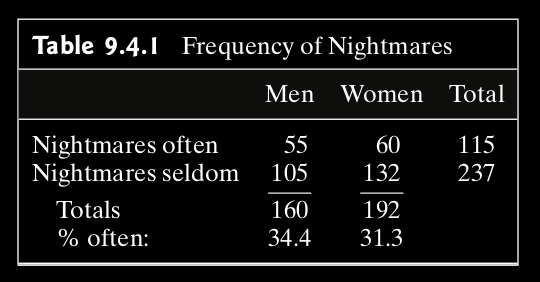
\includegraphics[scale=0.25]{Table_9-4-1-neg.png}
\end{center}
Is 34.4\% significantly different from 31.1\% ($\alpha=0.05$)?
\vfill
\item[Sol.] ... \myEnd
\end{enumerate}
\end{frame}
%-------------- end slide -------------------------------%}}}
